\subsection{Historical GP search diagnostics}\label{app:historical-search}

Historical GP target scores provide a separate view in the first panel of
\cref{fig:fw-target-progress}. The 159 repeated dataset/cut/arm groups cover
55 distinct dataset/cut pairs; the 64 groups with lower final scores cover
23 pairs. Shared incumbent and teacher seeds make the arms dependent.
Scope: \cref{sec:method-status}.

The remaining three panels of \cref{fig:fw-target-history} follow one
historical dataset/cut, chosen after inspection for the largest
policy-seeded relative improvement in the preceding comparison set. Every
reported generation is shown, without applying a cumulative minimum. All
three arms finish at the same value; the policy-seeded arm first records it
one generation after the controls. Shared seeds prevent treating their
matching outcomes as independent discoveries.

\begin{figure*}[!t]
  \setlength{\abovecaptionskip}{4pt}
  \centering
  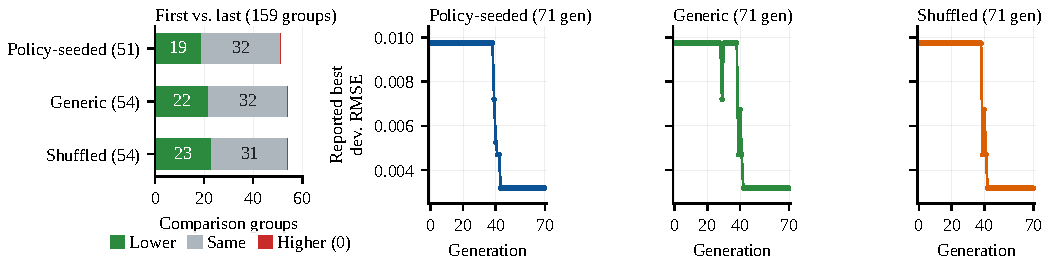
\includegraphics[width=\linewidth,height=1.50in,keepaspectratio]{figures/fig_fw_target_history.pdf}
  \caption{\textbf{Historical GP target progress and post-hoc 71-generation trajectories.}
  First panel: first-to-last reported best development RMSE across all 159 repeated comparison
  groups (55 distinct dataset/cut pairs) at \num{1000} evaluations per search, grouped by search arm.
  Second through fourth panels: all 71 generations per arm for one historical dataset/cut selected
  post hoc for the largest policy-seeded relative improvement. RMSE is in historical evaluator units
  (lower is better). The arms shared incumbent and teacher seeds, and elapsed time varied; these
  development records do not establish independent discoveries or a learned-policy advantage.}
  \label{fig:fw-target-progress}
  \label{fig:fw-target-history}
\end{figure*}
